Un algorithme partitionné nécessite le démarrage des tâches sur un processeur en particulier. Par exemple, j'ai ici démarré deux taches \texttt{rtspin} avec \textit{liblitmus} : l'une à un pire temps d’exécution de 2ms et une période de 5ms tandis que l'autre a un pire temps d’exécution de 4ms et une période de 7ms.

\begin{figure}[H]
    \centering
    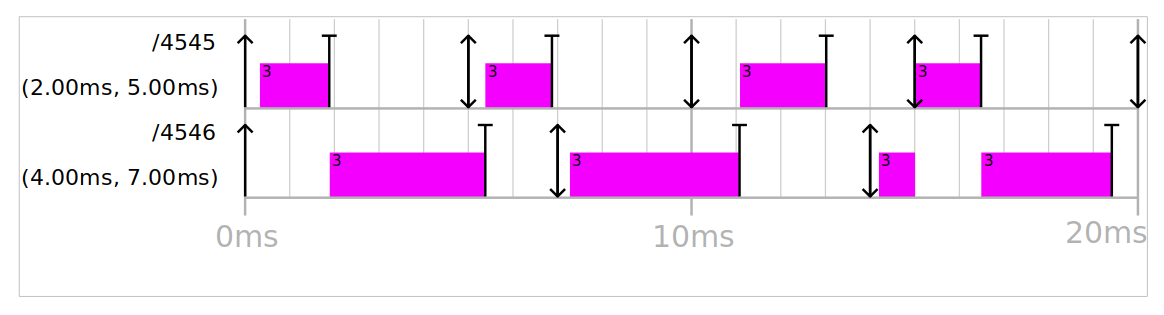
\includegraphics[width=0.5\paperwidth]{Images/P-EDF-SCHEDUALIBILITY-DEMO.png}
    \caption{Ordonnancement de deux taches avec P-EDF}
\end{figure}

On peut voir que a $t=5ms$, il n'y a pas préemption de la première tâche et la seconde termine son éxécution. En effet, selon EDF, la deuxième tâche à une \textit{deadline} dans 2ms, tandis que la première a une \textit{deadline} dans 5ms : la seconde est donc a cet instant plus prioritaire que la première. Cependant, à $t=15ms$, la seconde tâche est préemptée par la première car cette dernière se réveil et a une \textit{deadline} dans 5ms tandis que la seconde a une \textit{deadline} dans 6ms. On peut alors voir que la seconde tâche est préemptée à $t=15ms$ et reprend son exécution à $t=17ms$. 